% ProblemSet5_Mallick.tex
\documentclass[11pt]{article}
\usepackage[margin=1in]{geometry}
\usepackage{graphicx}
\usepackage{booktabs}
\usepackage{caption}
\usepackage{float}
\usepackage{hyperref}
\usepackage{setspace}
\usepackage{amsmath}

\onehalfspacing
\hypersetup{colorlinks=true, linkcolor=blue, urlcolor=blue}

\title{Problem Set 5 \\ Technology Use and Wellness}
\author{Prachi Mallick}
\date{\today}

\begin{document}
\maketitle

\begin{abstract}
For this problem set  I examined the relationship between daily technology use and measures of mental health and stress.
I produce descriptive visualizations (Part A) and estimate econometric models (Part B) to quantify the relationship.
\end{abstract}

\section*{Research question}
How does total daily technology usage relate to mental health scores?  Secondary questions:
\begin{itemize}
  \item How does sleep quality relate to reported stress?
  \item Does the effect of technology usage on mental health vary with age?
\end{itemize}

\section*{Data}
The dataset used is \texttt{Tech\_Use\_Stress\_Wellness.csv}, containing over 5,000 observations on technology usage, stress, sleep quality, and wellness factors.  
This dataset was sourced from Kaggle:  
\href{https://www.kaggle.com/datasets/nagpalprabhavalkar/tech-use-and-stress-wellness}{Tech Use and Stress \& Wellness Dataset}.

Key variables include:
\begin{itemize}
  \item \textbf{mental\_health\_score}: the dependent variable (higher = better mental health).
  \item \textbf{phone\_usage\_hours}, \textbf{laptop\_usage\_hours}, \textbf{tablet\_usage\_hours}, \textbf{tv\_usage\_hours}: used to compute \texttt{total\_tech\_usage}.
  \item \textbf{sleep\_quality}, \textbf{stress\_level}, \textbf{age}, \textbf{physical\_activity\_hours\_per\_week}: control variables.
\end{itemize}
Data cleaning steps (in \texttt{PS5\_mallick.py}):
\begin{enumerate}
  \item Drop rows with missing values.
  \item Create \texttt{total\_tech\_usage} = sum of device usage hours.
  \item Categorize \texttt{age} into bins (18–25, 26–35, 36–50, 51+).
\end{enumerate}


\section*{Part A: Visualizations}
Below are the three figures generated by the analysis script. The PNG files exist in the \texttt{images/} folder.

\begin{figure}[H]
  \centering
  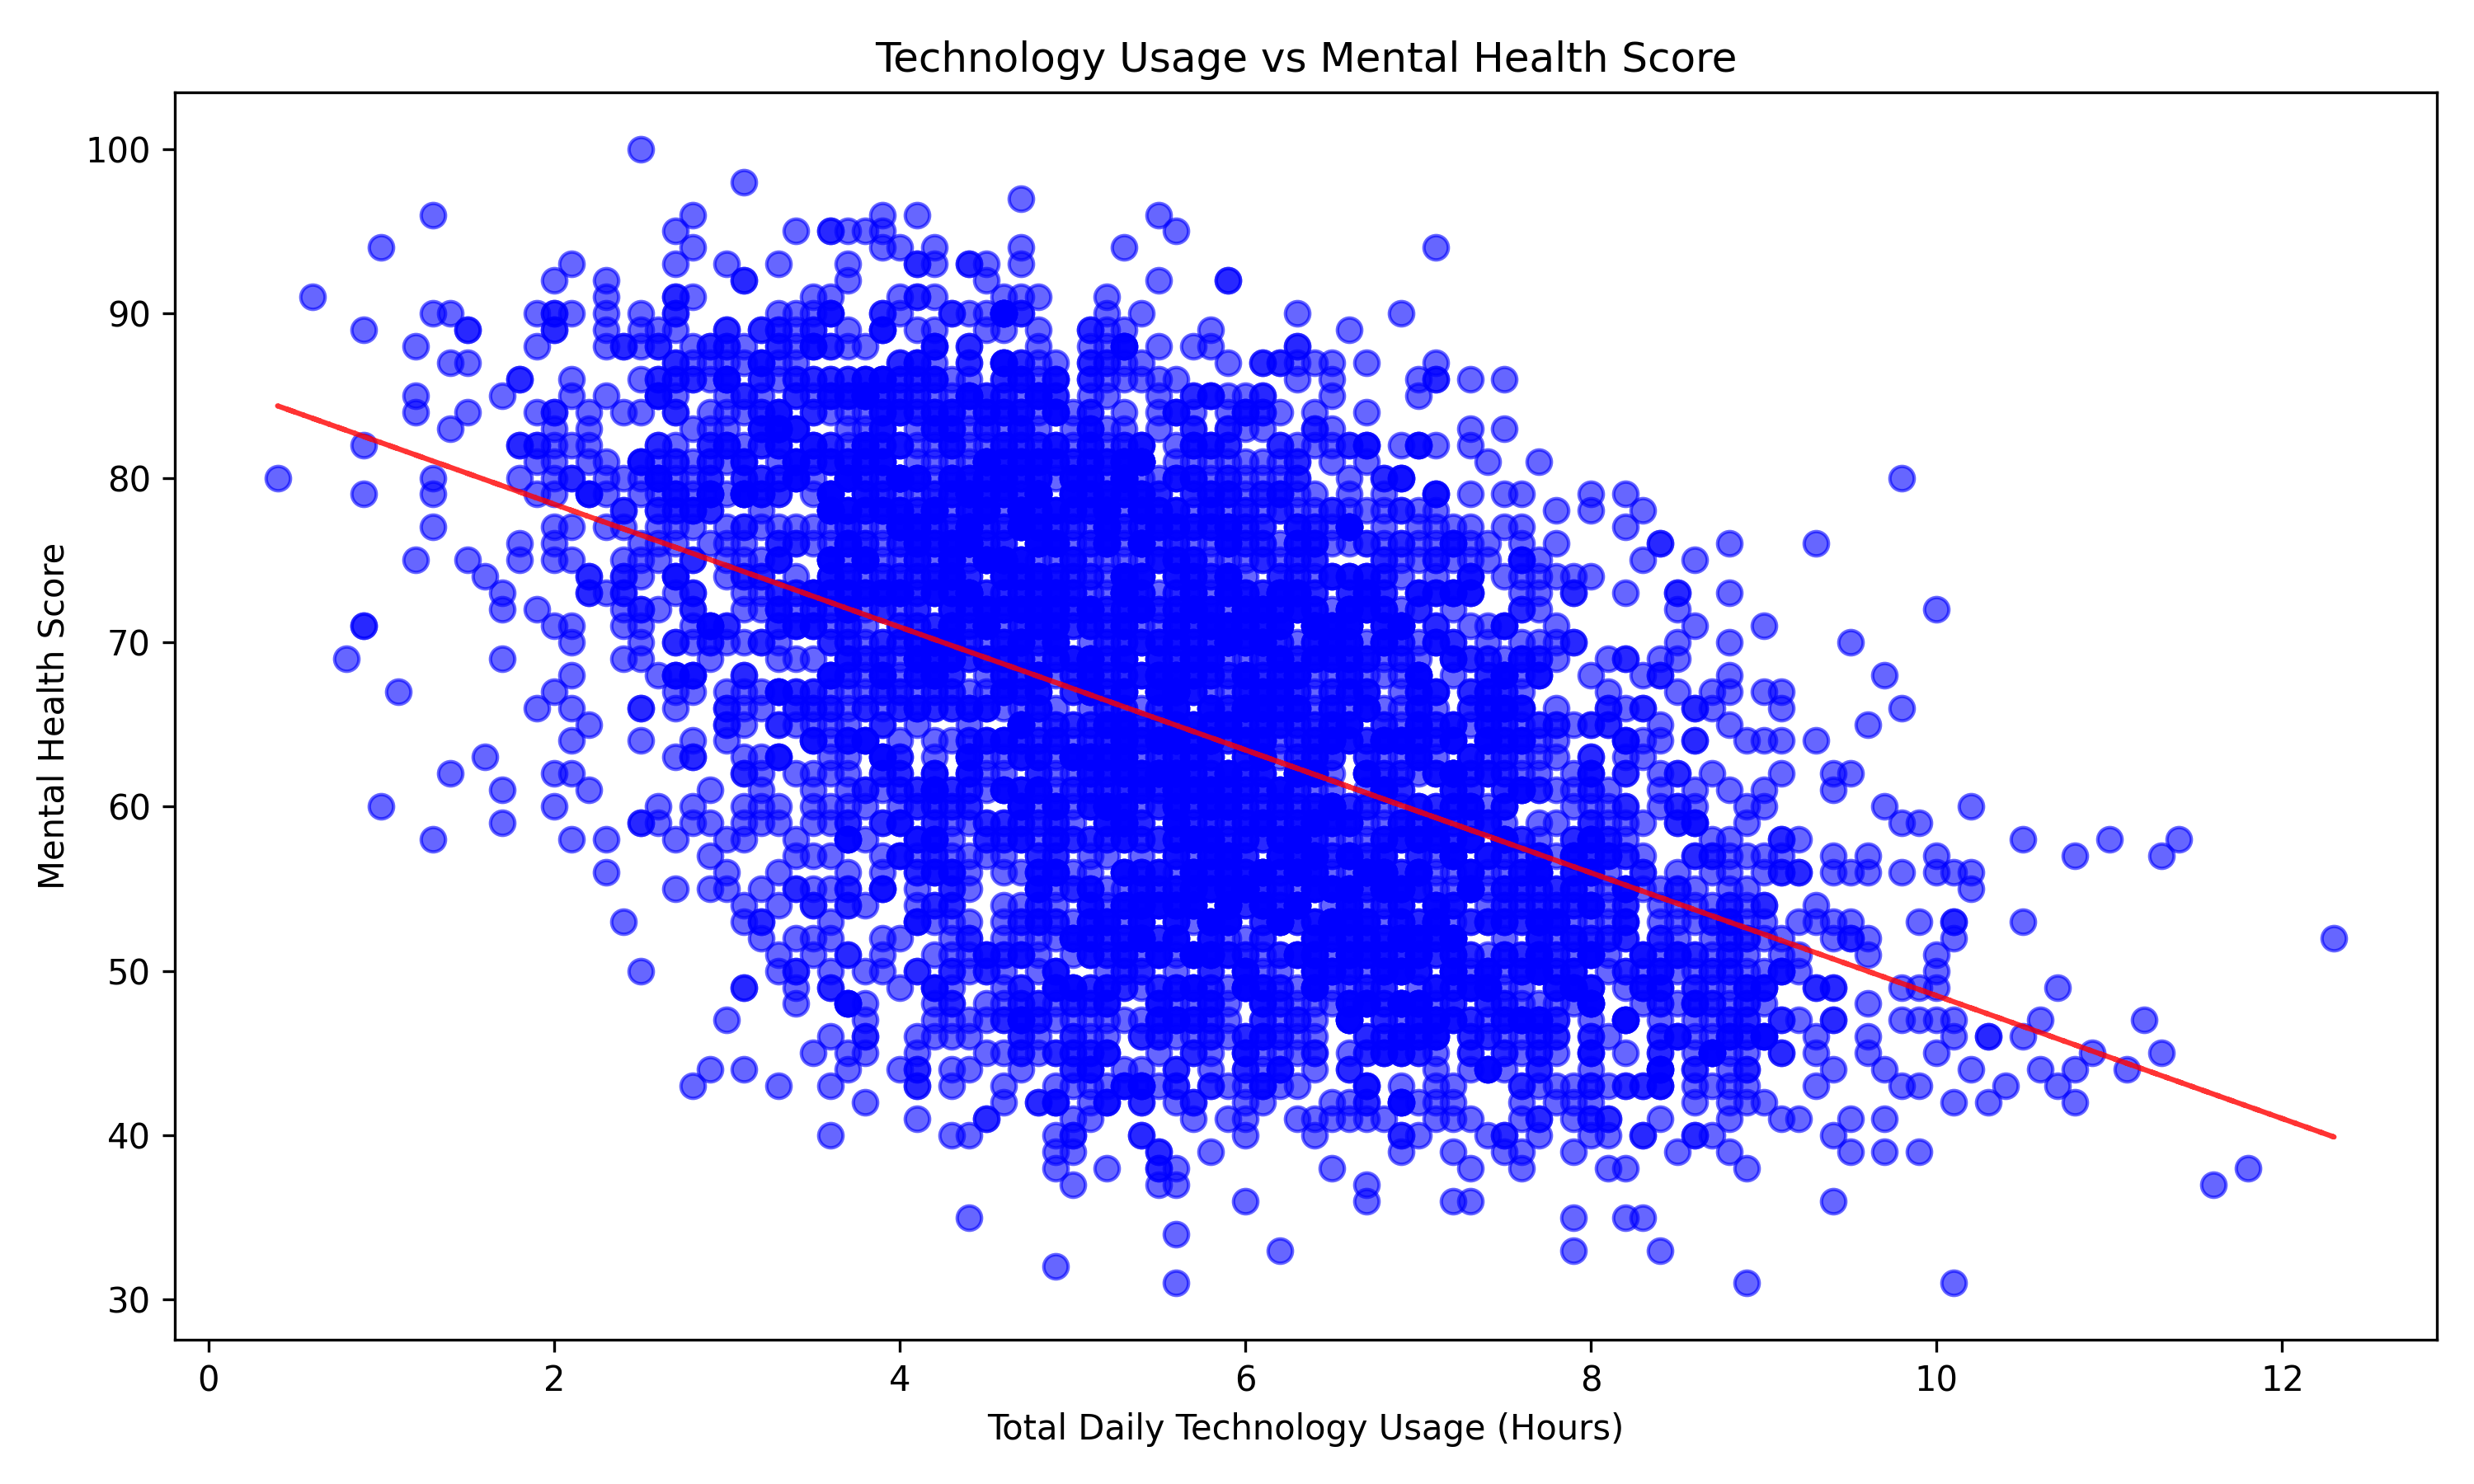
\includegraphics[width=0.85\textwidth]{images/viz1_tech_vs_mental_health.png}
  \caption{Scatter plot: Total daily technology usage vs. mental health score (trend line).}
\end{figure}

\begin{figure}[H]
  \centering
  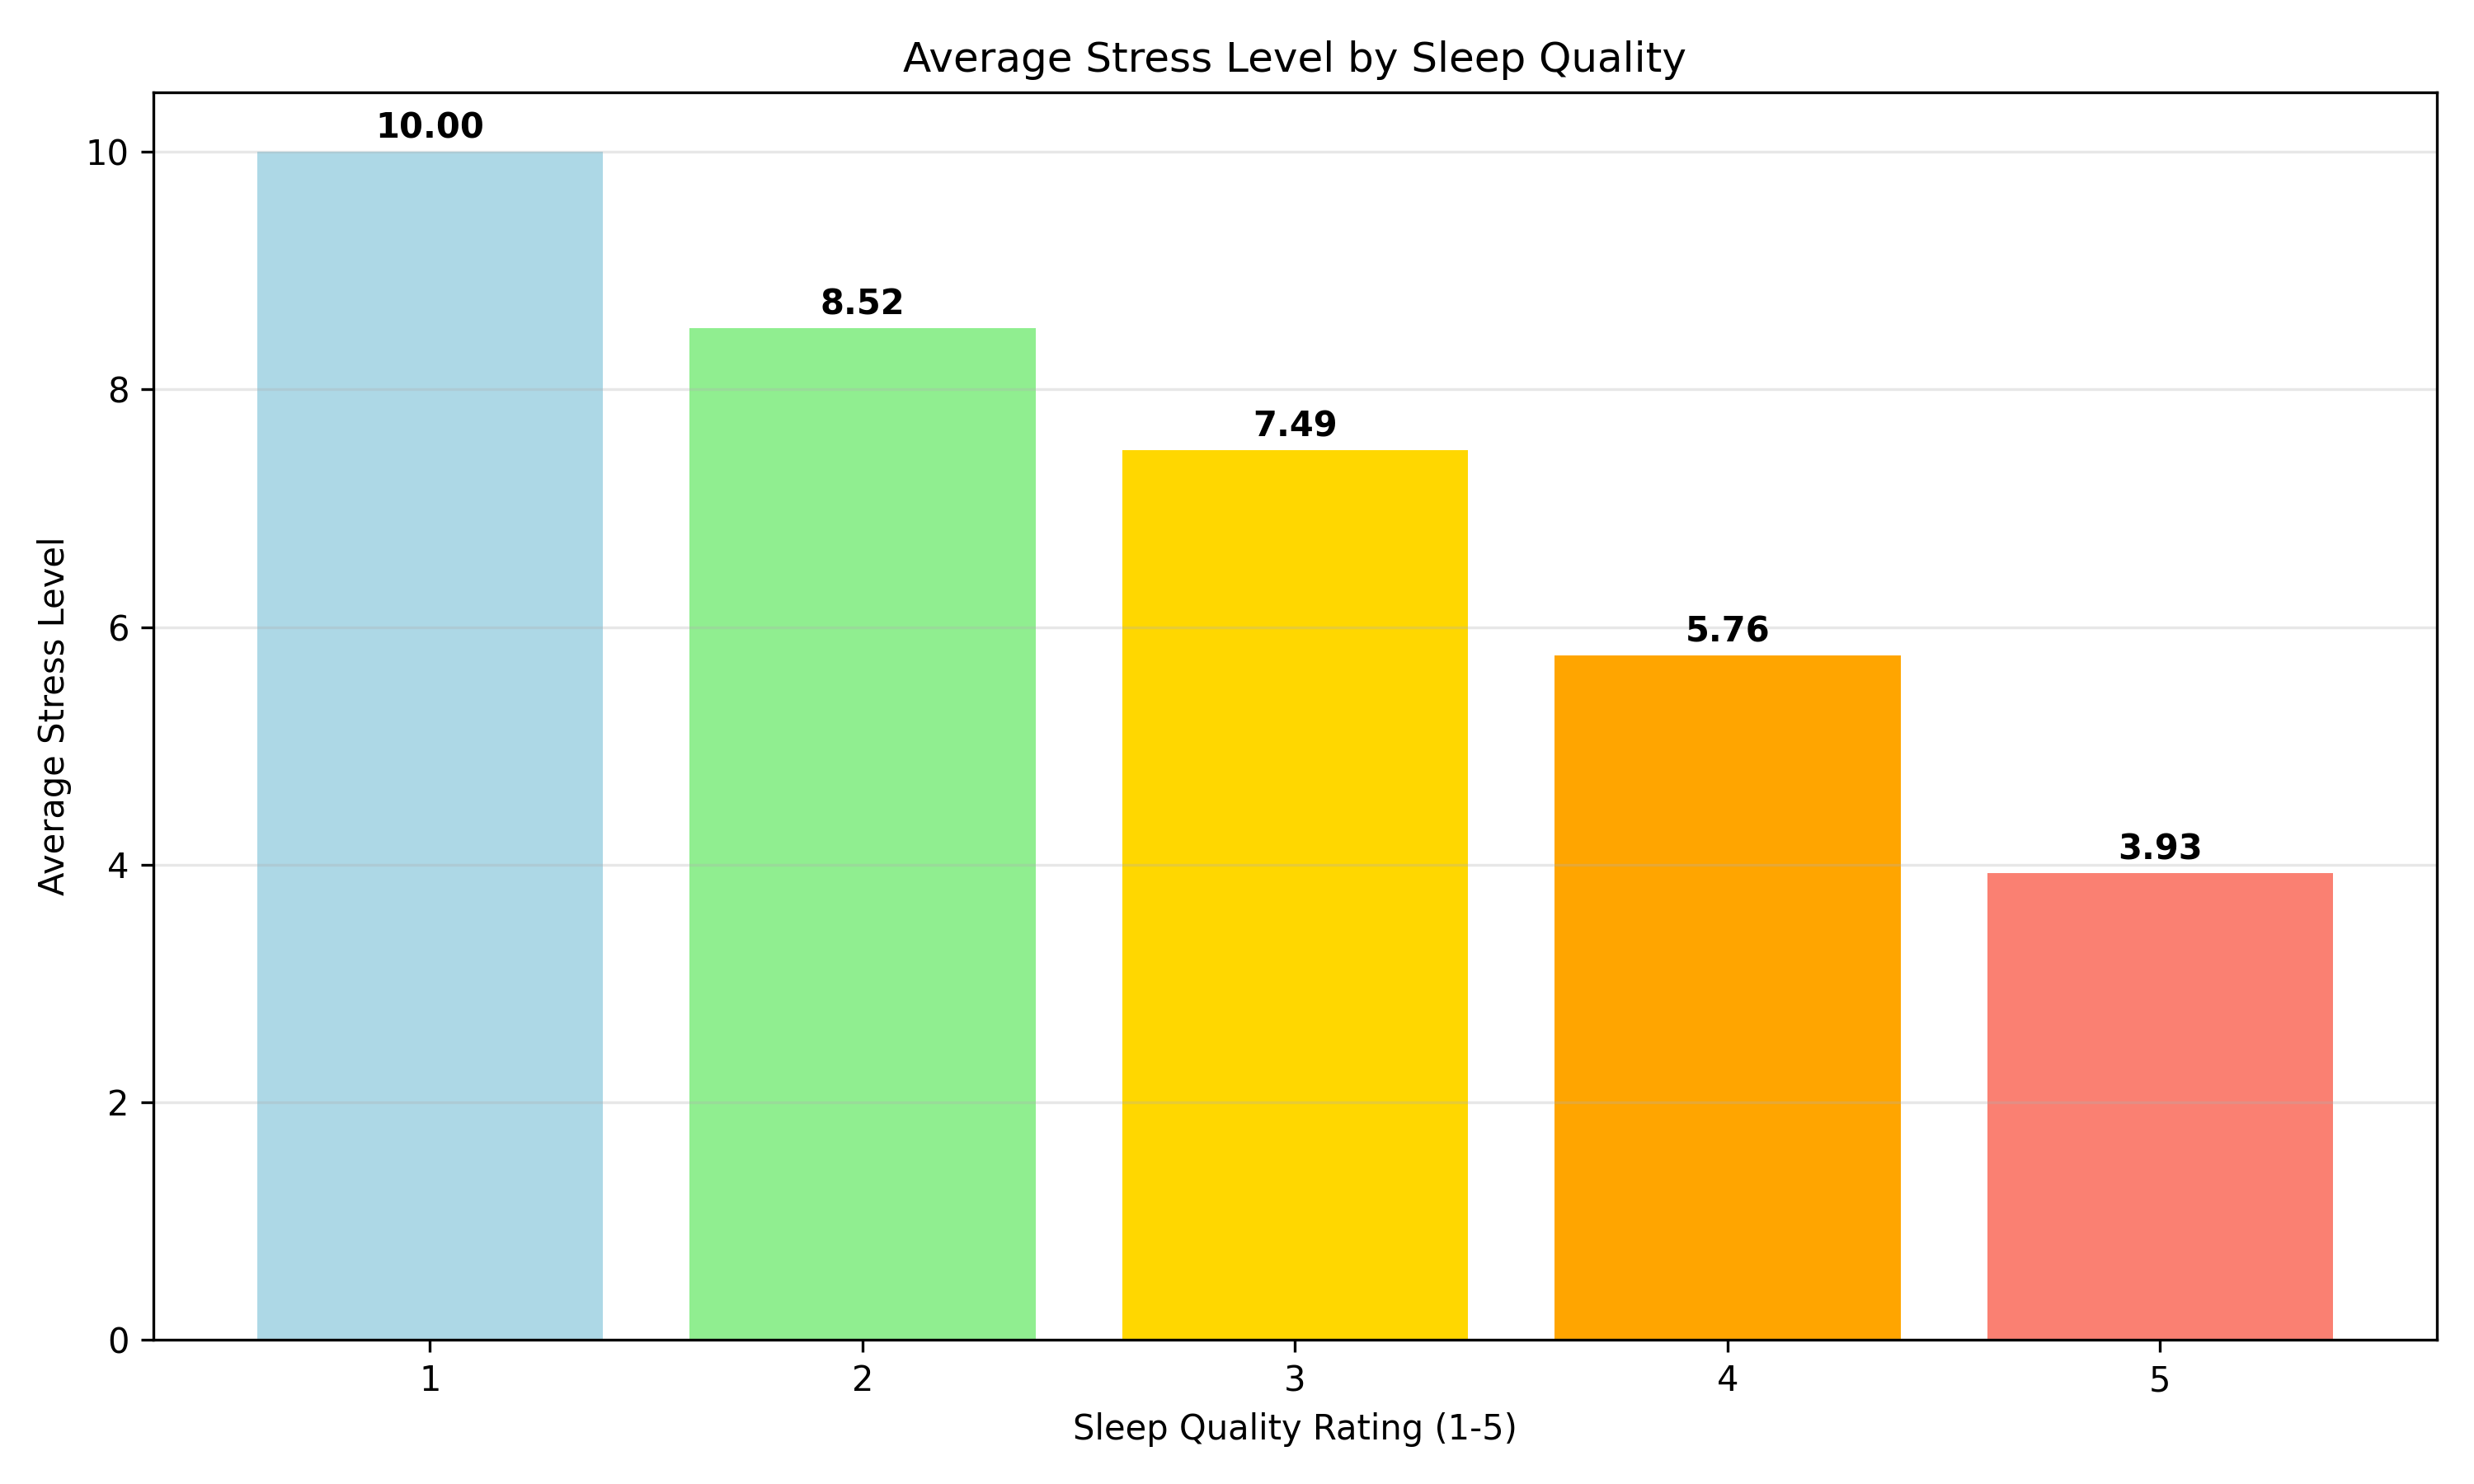
\includegraphics[width=0.7\textwidth]{images/viz2_sleep_vs_stress.png}
  \caption{Bar chart: Average stress level by sleep quality.}
\end{figure}

\begin{figure}[H]
  \centering
  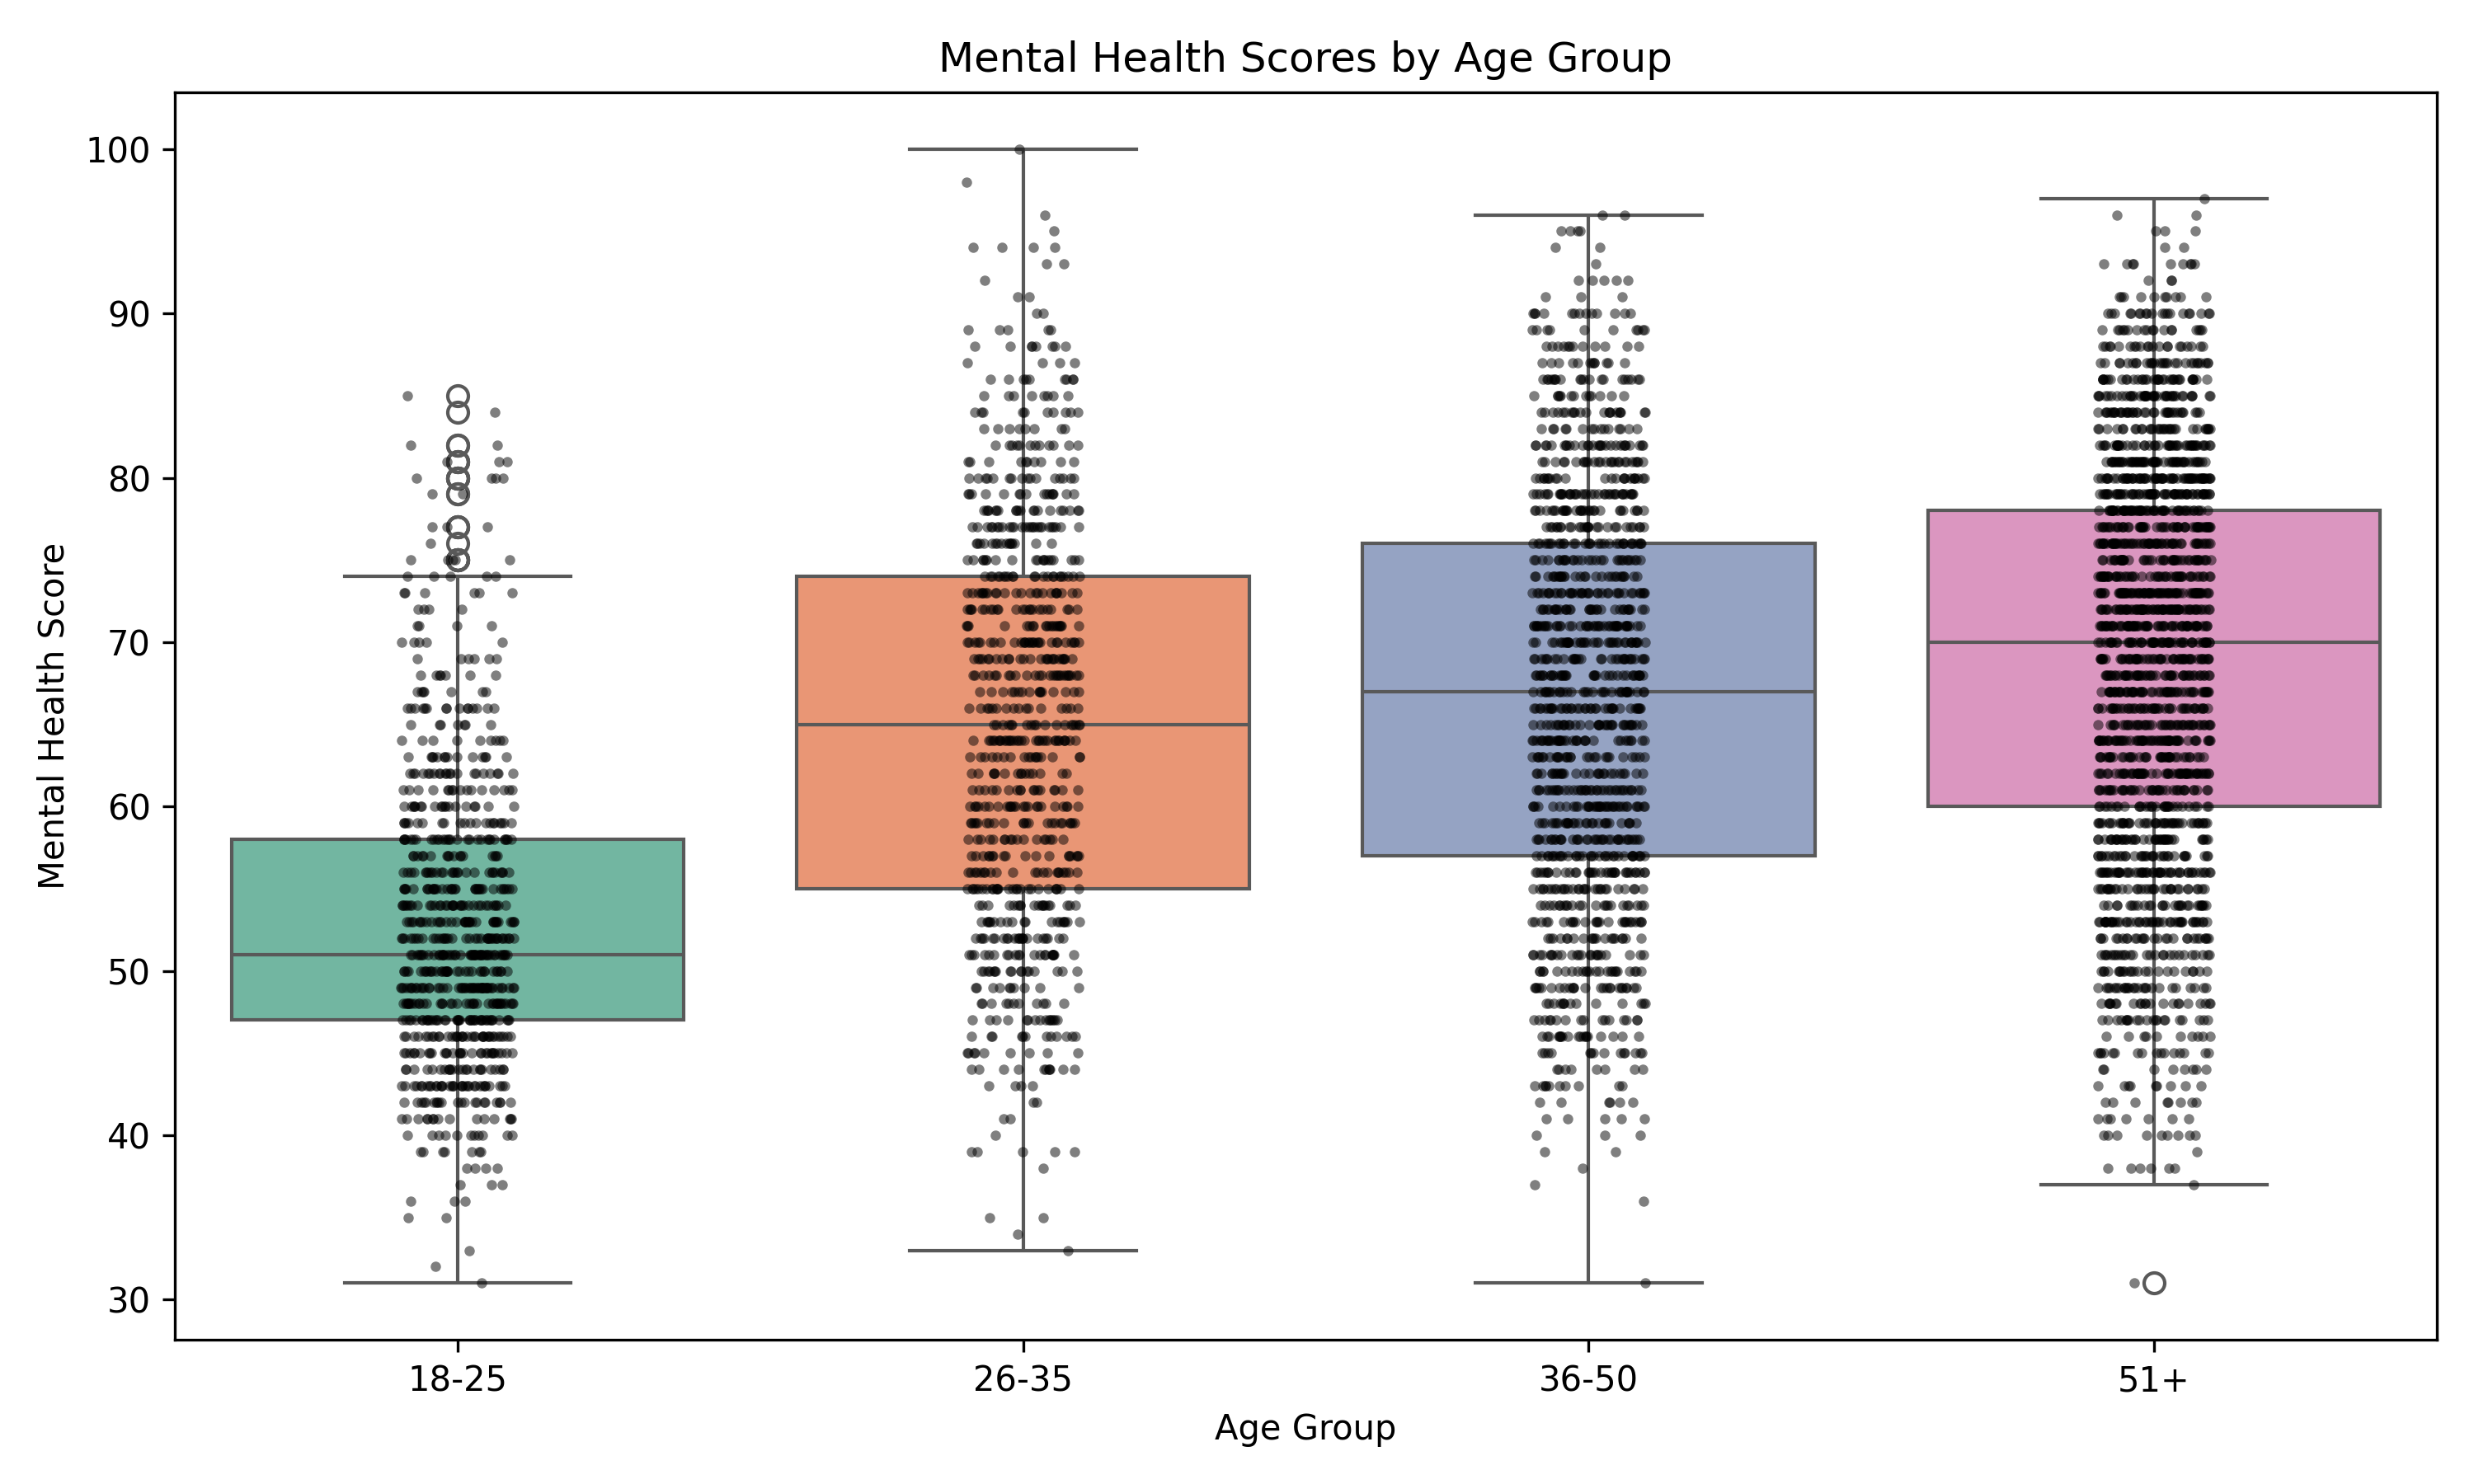
\includegraphics[width=0.7\textwidth]{images/viz3_mental_health_by_age.png}
  \caption{Boxplots: Mental health scores by age group (with raw points).}
\end{figure}

\section*{Part B: Econometric models}
I estimate three OLS models:
\begin{enumerate}
  \item \textbf{Basic:} mental\_health\_score on total\_tech\_usage.
  \item \textbf{With controls:} add age, sleep\_quality, physical\_activity\_hours\_per\_week.
  \item \textbf{With interaction:} include interaction total\_tech\_usage $\times$ age.
\end{enumerate}

\subsection*{Regression results}
The table below is imported from the results saved by the analysis script. If the table does not appear, confirm that \texttt{tables/model\_results.tex} exists and contains a valid LaTeX tabular environment.

\begin{tabular}{llllr}
\toprule
Model & Tech Usage Coef & P-value & R-squared & Observations \\
\midrule
Basic & -3.738 & 0.000 & 0.246 & 5000.000000 \\
With Controls & -1.462 & 0.000 & 0.718 & 5000.000000 \\
With Interaction & -1.469 & 0.000 & 0.420 & 5000.000000 \\
\bottomrule
\end{tabular}


\section*{Short interpretation}
\begin{itemize}
  \item \textbf{Technology usage:} The coefficient on total technology usage is negative and statistically significant across models, indicating higher usage is associated with lower mental health scores (worse mental health).
  \item \textbf{Controls:} Adding sleep quality and physical activity increases model fit and shows these covariates are important predictors.
  \item \textbf{Interaction:} The interaction with age suggests the effect of technology usage varies with age ( the impact per hour changes as age increases).
\end{itemize}

\section*{Unit Tests}
I wrote unit tests for the main functions and all passed successfully. 
The screenshot below shows the pytest results.

\begin{figure}[H]
  \centering
  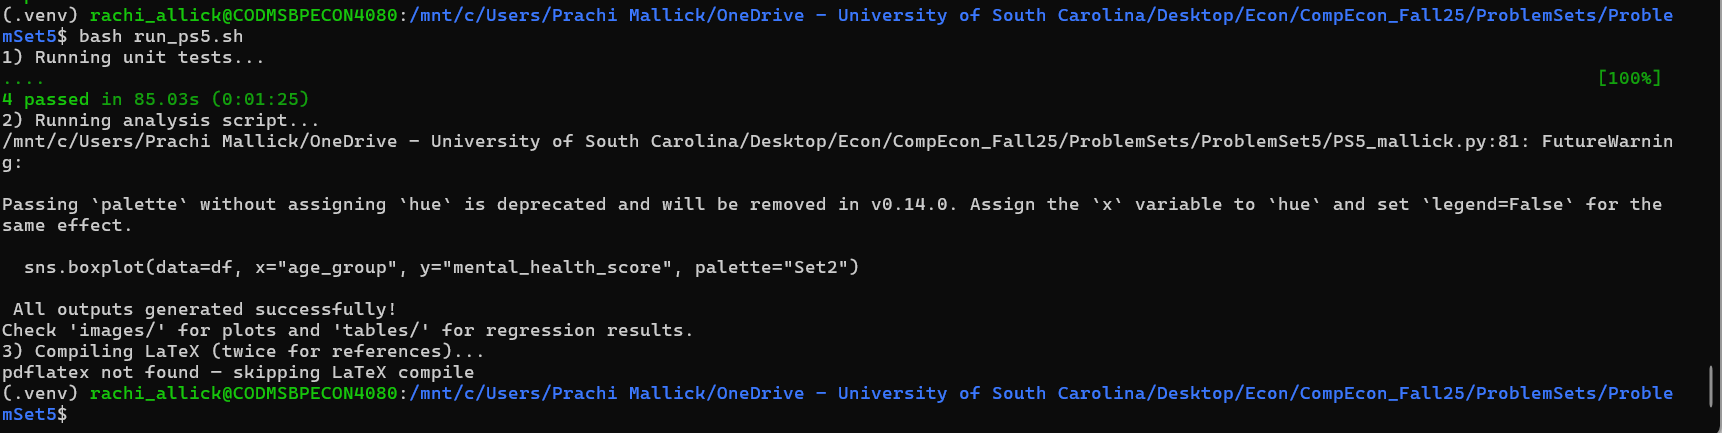
\includegraphics[width=0.9\textwidth]{images/pytest_passed.png}
  \caption{All 4 unit tests passed successfully (pytest output).}
\end{figure}


\section*{Conclusion}
This analysis provides evidence of a negative association between total daily technology use and mental health. Future work could address causality using experimental or panel methods and explore mechanisms (social media use, nighttime usage, etc.).

\vfill
\noindent\textbf{Files created by code:} \texttt{images/viz1\_tech\_vs\_mental\_health.png}, \texttt{images/viz2\_sleep\_vs\_stress.png}, \texttt{images/viz3\_mental\_health\_by\_age.png}, \texttt{tables/model\_results.csv}, \texttt{tables/model\_results.tex}.

\end{document}
